% Elegimo el tipo de documento y las características más importantes
\documentclass[a4paper,12pt]{article}

% Importación de los diferentes paquetes que se usan en el documento
\usepackage[colorlinks=true,linkcolor=black,urlcolor=black,breaklinks=true,citecolor=black]{hyperref}
\usepackage[spanish, es-tabla]{babel} 
\usepackage[labelfont=bf]{caption} % nombre captions en negrita
\usepackage[table,xcdraw]{xcolor}  % para las tablas
\usepackage[utf8]{inputenc}        % codificación de caracteres en español
\usepackage{multirow, array}       % para las tablas
\usepackage{tocbibind}             % para incluir bibliografía en índice
\usepackage{scrextend}             % tamaño de letra
\usepackage{booktabs}              % para las anotaciones
\usepackage{appendix}              % apéndice
\usepackage{graphicx}              % imágenes
\usepackage{listings}              % para las listas y el código integrado
\usepackage{fancybox}              % para los marcos de las portadas
\usepackage{setspace}
\usepackage{fancyhdr}              % para los encabezados de las paginas
\usepackage{parskip}               % para la configuración de los párrafos
\usepackage{anysize}               % para los margenes de pagina
\usepackage{eurosym}
\usepackage{courier}               % usar letra courier con \texttt{}
\usepackage{wrapfig}               % para los tamaños y posiciones de las imágenes
\usepackage{float}                 % para mantener el orden en las imágenes
\usepackage{cite}                  % para las referencias dentro del documentos
\usepackage{tabu}

\setlength{\columnsep}{0.5cm}

\definecolor{shadecolor}{rgb}{1,1,1}

% seteamos unos comandos para automatizar funciones
\renewcommand{\lstlistingname}{Código}  % Renombra listado códigos
\renewcommand\appendixtocname{Anexos}   % Renombra appendix a apéndices en índice
\renewcommand\appendixpagename{Anexos}  % Renombra appendix a apéndices en página

% \renewcommand{\insertImage}[4]
%{
 %\begin{figure}[H]
    %\centering
    %\includegraphics[scale={#4}]{{#1}}
    %\caption{{#2}}
    %\label{{#3}}
%\end{figure}
%}
% \insertImage{imagenes/diseno/epicasHistorias.png}{Relación entre épicas y temas}{fig:epicasHistorias}{0.6}

\singlespace

% setamos los tama;os y maregnes de las paginas
\marginsize{1.5cm}{2cm}{1.5cm}{2cm} % {izdo}{dcho}{arriba}{abajo}
\parindent=0,5cm

% seteamos el encabezado y los pies de las paginas
\renewcommand{\headrulewidth}{0.5pt}
\renewcommand{\footrulewidth}{0.5pt}
\pagestyle{fancy} 

\lhead[UVa]{UVa}
\rhead[Trabajo Fin Grado]{Trabajo Fin Grado}

\lfoot[Aplicación base datos pigmentos]{Aplicación base datos pigmentos}
\cfoot[]{}
\rfoot[\thepage]{\thepage}

% seteamos la configuracion del codigo integrado 
\definecolor{mygray}{rgb}{0.95,0.95,0.95}

\lstdefinestyle{customc}{
	backgroundcolor=\color{mygray},
	frame=single,
	keepspaces=true,
	keywordstyle=\color{blue},
	commentstyle=\color{magenta},	
	language=c,
	numbers=left,
	numbersep=25pt,
	numberstyle=\color{black}
}


\begin{document}

%introducimos las portadas, tanto exterior como interior
% PORTADA EXTERIOR
\begin{titlepage}

% imagen superior
\begin{center}
\thisfancypage{\setlength{\fboxsep}{20pt}\doublebox}{}
\begin{figure}[htb]
\begin{center}

\includegraphics[scale=0.5]{imagenes/logo.jpg}
\end{center}
\end{figure}

\begin{LARGE}
\textbf{Universidad de Valladolild}
\end{LARGE}

\vspace*{0.8in}
\begin{Huge}
\textbf{Escuela de Ingeniería Informática}
\end{Huge}

\vspace*{0.4in}
\begin{Large}
\textbf{TRABAJO DE FIN DE GRADO}
\end{Large}

\vspace*{1in}
\begin{LARGE}
Grado en Ingeniería Informática, Mención en Tecnologías de la Información y de la Comunicación
\end{LARGE}

\vspace{0.6in}
\begin{Huge}
\textbf{Desarrollo de una aplicación móvil para la explotación de una base de datos de pigmentos}
\end{Huge}

\vspace{0.6in}
\begin{flushright}
\begin{Large}
Autor:\\
\textbf{Sergio Esteban Pellejero}
\end{Large}
\end{flushright}
\end{center}
\end{titlepage}

% PORTADA INTERIOR
\begin{titlepage}
\begin{center}
\thisfancypage{\setlength{\fboxsep}{20pt}\doublebox}{}
\begin{figure}[htb]
\begin{center}

\includegraphics[scale=0.5]{imagenes/logo.jpg}
\end{center}
\end{figure}

\begin{LARGE}
\textbf{Universidad de Valladolild}
\end{LARGE}

\vspace*{0.8in}
\begin{Huge}
\textbf{Escuela de Ingeniería Informática}
\end{Huge}

\vspace*{0.4in}
\begin{Large}
\textbf{TRABAJO DE FIN DE GRADO}
\end{Large}

\vspace*{0.8in}
\begin{LARGE}
Grado en Ingeniería Informática, Mención en Tecnologías de la Información y de la Comunicación
\end{LARGE}

\vspace{0.6in}
\begin{Huge}
\textbf{Desarrollo de una aplicación móvil para la explotación de una base de datos de pigmentos}
\end{Huge}

\vspace{0.4in}
\begin{flushright}
\begin{Large}
Autor:\\
\textbf{Sergio Esteban Pellejero}\\
Tutor:\\
\textbf{Joaquin Adiego}
\end{Large}
\end{flushright}

\end{center}
\end{titlepage}
% fin de las portadas



% introducimos el resumen, tanto en español como en ingles
\begin{abstract}
\setlength{\parskip}{0.5cm}

El fin de este trabajo de fin de grado es recrear una antigua página web que explotaba una base de datos orientada a la pigmentación. La aplicación antigua hecha en forma de web ha sido trasladada a una aplicación móvil capaz de ejecutarse en cualquier dispositivo con Android que hay en la actualidad. 

Primero se ha tenido que recuperar la información existente desde un dispositivo de almacenamiento antiguo, como un CD. Una vez analizada la poca documentación actual y revisada la estructura de la base de datos, se ha procedido a trasladarla a una base de datos más actual, en este caso se ha decidido usar una base de datos SQLite. Una vez hemos diseñado e implementado la base de datos de la manera correcta, se ha procedido a desarrollar la aplicación móvil. En este caso se ha decidido usar Java como lenguaje de programación por la familiaridad del lenguaje a la hora de programar. 

Cabe destacar que la metodología que se ha implementado para llevar a cabo este trabajo refleja un poco la de Kanban, ya que el proyecto se ha apoyado en una herramienta de gestión de proyectos de código abierto y libre como es Taiga.io, donde se puede ver todo el desarrollo, fechas y tiempo del proyecto, junto con los problemas que se han ido teniendo y solucionando. 

Como consecuencia de la metodología utilizada, se han mezclado las fases de desarrollo con las fases de diseño, además de que no todas las partes de diseño se ven cubiertas de manera completa. 
\end{abstract}
\begin{abstract}
\setlength{\parskip}{0.5cm}
\end{abstract}

\newpage

% introducimos todas las listas, tanto el índice, como la de figuras y tablas
\tableofcontents
\listoffigures
\newpage

% acabamos de decidir algunas configuraciones para el resto del documento
%\changefontsizes[16pt]{12pt}
\pagenumbering{Roman}
\hypersetup{linkcolor=black}
\newpage
\pagenumbering{arabic}

% empezamos a escribir el documento como tal con toda la información relevante
\section{Diseño de la base de datos}
\setlength{\parskip}{0.5cm}

En esta sección vamos a mostrar como se ha llevado a cabo el diseño de la base de datos y los diferentes procedimientos utilizados. 

Tenemos que destacar que contamos con una implementación de la base de datos de pigmentos. El problema es que dicha base de datos esta implementada en AccessDB, que es un sistema gestor de bases de datos propietario de Microsoft. Existen herramientas que permiten la integración de dichos tipos de bases de datos en otros gestores como MySQL o SQLite.

En este caso la base de datos se va a diseñar desde 0 para una mejor optimización de los recursos, además se utilizará como sistema gestor de bases de datos SQLite, ya que tiene una integración completa de serie con los terminales Android.

\subsection{Suposiciones y convenciones}
En este apartado se van a aclarar ciertas cosas acerca de los identificadores de las relaciones, formatos que hemos decidido usar y algunas otras convenciones que me parece apropiado comentar en relación al diseño de la base de datos. 

\begin{itemize}
    \item Los identificadores tanto de los pigmentos, que actúan como clave primaria de la mayoría de las relaciones quedan representados por el descriptor breve. En este caso el descriptor es un código numérico que se ira generando de manera automática en la base de datos. De esta forma nos aseguramos de que cada uno de los pigmentos y de los datos relacionados están representados de manera unívoca por un número identificativo. 
    \item Cabe destacar que en el diagrama de entidad relación el formato que se ha seguido para representar las cardinalidades de las relaciones queda representado por el formato típico de UML, y no el que dicta el diseño propio de las bases de datos convencionales. 
\end{itemize}

\subsection{Posibles consultas contra la BBDD}
Vamos a analizar de manera breve las diferentes consultas que podemos realizar contra la base de datos que tenemos que diseñar. En nuestro caso, las consultas quedan determinadas por las diferentes interfaces que vamos a tener en nuestra aplicación. En este caso la principal información que vamos a tener que extraer de la base de datos es la siguiente:

\begin{itemize}
    \item Información acerca de cada uno de los pigmentos: en nuestra aplicación tenemos una vista en la que se muestra una lista con todos los pigmentos junto con la información más básica de cada uno de ellos, como puede ser el nombre, el color y el elemento químico principal por el que están compuestos. Esta información la podemos extraer directamente de la relación Pigmentos, donde tenemos toda la información básica de todos ellos. 
    \item Coordenadas colorimétricas: cada uno de los pigmentos consta de una serie de coordenadas que determinan el color y la luminosidad del mismo. Estas coordenadas serán almacenadas en una relación diferente porque la considero una característica un poco más avanzada que por ejemplo el nombre del pigmento. Cada uno de los pigmentos tendrá una relación directa con sus coordenadas colirimétricas. Esta relación será posible gracias al identificador único del pigmento que será utilizado como clave primaria en todas las relaciones. 
    \item Difractograma de rayos X: cada uno de los pigmentos tiene información relacionada con su generación del difractograma de rayos X característico. Por ello esta información se ha almacenado en una tabla diferente y el método de acceso será equivalente al mencionado en la relación anterior. Tenemos que ser capaces de extraer una gráfica para poder mostrar el espectro de rayos X de cada uno de los elementos que tenemos en la base de datos. 
    \item Infrarojos: otra de las características representativa de cada uno de los pigmentos es su \textcolor{red}{mirar en la documentación las definiciones exactas de cada una de las cosas que estoy poniendo} espectro de infrarojos, básicamente va a estar compuesto por dos valores a partir de los cuales se podrán generar una serie de gráficas. Tenemos que ser capaces de extraer las gráficas correspondientes al espectro de infrarojos para cada uno de los pigmentos.
    \item Espectro de Raman: cada uno de los pigmentos tiene asociado un espectro de Raman característico. Este espectro se puede generar gracias a dos valores, ya que es una gráfica simple, en la que luego tenemos que dar los puntos más representativos. Tenemos que ser capaces de extraer los 3 picos de Raman más importantes junto con las gráficas correspondientes. 
\end{itemize}

\subsection{Modelado conceptual}
\subsubsection{Entidades y atributos}

Las diferentes entidades junto con sus atributos son las siguientes: \textcolor{red}{mirar la definición de cada uno de los atributos de las entidades, además de mirar bien las relaciones}
\begin{itemize}
    \item \textbf{Pigmento}: tenemos que almacenar de una manera segura y persistente la información relacionada con cada uno de los pigmentos. Para ello simplemente vamos a exportar dichos datos de las bases de datos ya existentes y creadas en AccessDB. La información que tenemos que almacenar de cada uno de los pigmentos es la siguiente:
        \begin{itemize}
            \item \textit{Nombre}: nombre con el que se identifica a cada uno de los pigmentos dentro de la base de datos. Dicho nombre es único para cada uno de los pigmentos.
            \item \textit{Id Color}: id representando el color principal de cada uno de los pigmentos
            \item \textit{Notas}: los pigmentos pueden o no tener notas adjuntas, de hecho se permite a los usuarios añadir notas sobre dichos pigmentos. Es por ello que se permiten almacenar notas separadas de cada uno de los elementos de la base de datos.
            \item \textit{Potencia}: \textcolor{red}{TODO}
            \item \textit{Lambda}: \textcolor{red}{TODO}
            \item \textit{Fórmula}: los pigmentos al estar compuestos por elementos naturales, tienen fórmulas químicas determinadas. Es un dato importante si queremos saber su composición o como van a reaccionar cuando están en presencia de cierto elementos químicos, también la mostraremos.
            \item \textit{Sinónimos}: los pigmentos pueden tener sinónimos a la hora de ser llamados. Es por esto que cada uno de ellos tendrá una relación con sus sinónimos. 
            \item \textit{Elemento químico}: cada uno de los pigmentos tiene un elemento químico predominante en su composición química. Tenemos que almacenarlo para mostrarlo cuando proporcionemos la información relacionada con el pigmento.
        \end{itemize}
        
    \item \textbf{Colorimetría}:
        \begin{itemize}
            \item \textit{L}: \textcolor{red}{TODO}
            \item \textit{a}: \textcolor{red}{TODO}
            \item \textit{b}: \textcolor{red}{TODO}
            \item \textit{X}: \textcolor{red}{TODO}
            \item \textit{Y}: \textcolor{red}{TODO}
            \item \textit{Z}: \textcolor{red}{TODO}
            \item \textit{\textcolor{red}{TODO}}: \textcolor{red}{TODO}
        \end{itemize}
        
    \item \textbf{Difractograma de rayos X}:
        \begin{itemize}
            \item \textit{x}: \textcolor{red}{TODO}
            \item \textit{y}: \textcolor{red}{TODO}
        \end{itemize}
        
    \item \textbf{Espectro de Raman}:
        \begin{itemize}
            \item \textit{x}: \textcolor{red}{TODO}
            \item \textit{y}: \textcolor{red}{TODO}
        \end{itemize}
        
    \item \textbf{Espectro de infrarrojos}:
        \begin{itemize}
            \item \textit{x}: \textcolor{red}{TODO}
            \item \textit{y}: \textcolor{red}{TODO}
        \end{itemize}
        
    \item \textbf{Notas}: el usuario tiene que ser capaz de escribir notas rápidas para sí mismo acerca de cada uno de los pigmentos. Es por ello que una de las opciones de la aplicación es almacenar notas de uno de los pigmentos seleccionados. Dichas notas podrán ser recuperadas con posterioridad por el usuario para ser editadas o borradas.
        \begin{itemize}
            \item \textit{Título}: cada una de las notas que almacenamos de un pigmento consta de un título, que no es único y va a tener una longitud limitada a 100 caracteres. Tiene que ser algo corto y determinado. Ya que lo primero que ser verá cuando mostremos la vista de las notas es el título y estarán ordenadas por la fecha de creación, por lo que la última nota creada es la que se mostrará por completo. 
            \item \textit{Valor}: el valor es la nota en sí. Lo que el usuario introduzca en el formulario de escritura. 
            \item \textit{Fecha}: la fecha no será necesario mostrarla al usuario, pero si que tiene sentido almacenarla en la base da datos para tener un histórico de creación de las mismas y luego poder recuperarlas en diferente orden por la aplicación.  
        \end{itemize}
        
    \item \textbf{Sinónimos}: cada uno de los pigmentos puede tener nombres diferentes con los que ha sido referenciado a lo largo del tiempo. Es por esto que tendremos un lista para cada uno de los pigmentos con todos los sinónimos que tenga. 
        \begin{itemize}
            \item \textit{Valor}: como cada uno de los sinónimos puede tener 0 o más sinónimos, he decidido hacer una relación separada para cada uno de los pigmentos. Sino otra forma es hacer un atributo sinónimo dentro de la entidad Pigmento conteniendo una lista separada por comas con todos los sinónimos, pero me parece una mejor opción hacer una relación separada. 
        \end{itemize}
\end{itemize}

Antes de mostrar el diagrama de entidad relación vamos a mostrar una pequeña tabla con las diferentes cardinalidades y entidades relacionadas. Podemos encontrar dicho gráfico en la \textbf{Figura \ref{fig:cardinalidades}}

\begin{figure}[H]
    \centering
    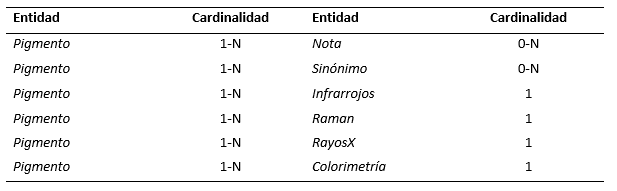
\includegraphics[scale=1]{imagenes/disenoBaseDatos/cardinalidades.png}
    \caption{Entidades y cardinalidades del modelo}
    \label{fig:cardinalidades}
\end{figure}

\subsubsection{Diagrama de Entidad Relación}

Una vez que hemos presentado tanto las entidades, como las cardinalidades y como están relacionadas las mismas, podemos mostrar como se relacionan las unas con las otras de una manera gráfica, que es presentado el diagrama de entidad relación de la base de datos. En este caso se ha decidido usar el formato de UML y no sigue las reglas estrictas del modelo de Entidad Relación, pero me parece que es más visual, la herramienta y el formato es más universal y entendible que el propio para expresar este tipo de contenidos. Podemos encontrar esto en la \textbf{Figura \ref{fig:diagramaER}}

\begin{figure}[H]
    \centering
    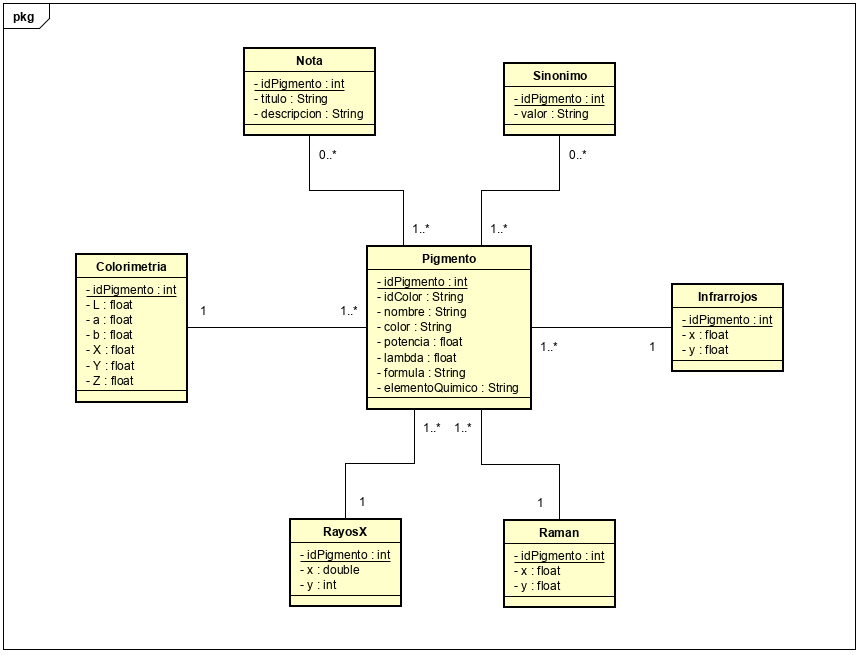
\includegraphics[scale=0.75]{imagenes/disenoBaseDatos/diagramaER.png}
    \caption{Diagrama de Entidad-Relación de la base de datos}
    \label{fig:diagramaER}
\end{figure}

En el diagrama podemos observar como la clave primaria de todas las relaciones es el id del pigmento en cuestión. Esto luego nos permitirá conectar unas relaciones con otras y buscar la información de una manera más adecuada. 

\textcolor{red}{mirar a ver las transformaciones y buscar un poco mas de teoría de diseño de la base de datos}

Una vez que tenemos el diseño de la base de datos podemos pasar a explicar la implementación de la misma, en lineas generales. 


\subsection{Implementación de la base de datos}
Una vez que tenemos la base de datos diseñada tenemos que implementarla dentro de nuestra aplicación. Para ello lo primero que tenemos que hacer es crear una clase auxiliar que nos permita la creación y en el futuro la conexión entre la propia aplicación y los datos almacenados en la base de datos. 

Para implementar la base de datos he optado por hacerlo de una manera más sencilla que la aprendida en la asignatura de SMOV. La base en realidad es la misma, pero la forma es la misma, bien es sabido que dentro de la informática podemos obtener los mismos resultados pero con algoritmos diferentes. En este caso vamos a realizar una mezcla entre uno de los patrones de acceso comentados al principio, DAO y los POJO.

Como hemos dicho en los capítulos anteriores, cada uno de los elementos de la base de datos, que en este caso son pigmentos, va a estar representado por un objeto típico de Java. Esta forma de representar los objetos para el almacenamiento de datos se denomina POJO (\textbf{P}lain \textbf{O}ld \textbf{J}ava \textbf{O}bjects).

Además cada vez que recuperemos los elementos de la base de datos lo hacemos devolviendo una lista de objetos del tipo adecuado. Por ejemplo para devolver todos y cada uno de los pigmentos que hay en la base de datos lo que hacemos es mandar la consulta al SGBD de SQLite y lo que nos devuelve es una lista de POJOs del tipo deseado. 

De esta manera podemos acceder de una manera sencilla a todos los atributos de los datos que acabamos de recuperar.

\subsubsection{¿Que son los POJO?} 

Dicho término \cite{pojo} fue acuñado por Martin Fowler, Rebecca Parsons y Josh MacKenzie en Septiembre del 2000. Se usa para referirse a un objeto Java que no tiene limitaciones de por requerir librerías ni clases externas. Son objetos simples y básicos de java, con atributos, funciones para recuperar los valores y para cambiarlos en caso necesario y nada más. Este tipo de objetos son muy utilizados cuando tenemos que convertir objetos entre diferentes lenguajes o cuando tenemos que serializarlos para enviarlos por la red. 

Idealmente y según dice la definición de los mismos, un objeto Java es POJO si cumple estos 3 requisitos:
\begin{itemize}
    \item No extiende de ninguna clase. 
        \begin{figure}[H]
        \lstinputlisting[style=customc]{capitulos/disenoBaseDatos/codigo/noExtiende.java}
        \label{fig:noExtiende}
        \end{figure}
    
    \item No implementa ninguna clase. 
        \begin{figure}[H]
        \lstinputlisting[style=customc]{capitulos/disenoBaseDatos/codigo/noImplementa.java}
        \label{fig:noImplementa}
        \end{figure}
        
    \item No contiene anotaciones. 
        \begin{figure}[H] 
        \lstinputlisting[style=customc]{capitulos/disenoBaseDatos/codigo/noAnotaciones.java}
        \label{fig:noAnotaciones}
        \end{figure}
\end{itemize}

Los POJO fueron inicialmente utilizados en J2EE para representar los JavaBeans, que son objetos java muy simples y que ofrecen servicios por la red. Se siguen utilizando aunque han cambiado un poco las formas de hacerlo. Ahora los POJO también son ampliamente utilizados para representar objetos JSON recibidos por parte de microservicios web y ser utilizados en un servidor. Este es uno de los muchos ejemplos de utilización real a día de hoy de los POJO. 

\subsubsection{Ejemplo}

Vamos a explicar con un sencillo ejemplo lo que son los POJO y como se hace la consulta de los mismos para luego mostrar la información dentro de la aplicación.

En este caso uno de los atributos que nos interesa son las diferentes notas que tiene cada uno de los pigmentos, para ello habrá una tabla con todas las notas de todos los pigmentos. Como hemos enseñado en el modelado conceptual, de cada una de las diferentes notas almacenamos y guardamos los siguientes datos: 
\begin{itemize}
    \item IdPigmento: para poder relacionar la nota con el pigmento, este dato es interno para la gestión de los datos. 
    \item Título: breve descripción.
    \item Descripción: contenido completo de la nota. 
    \item Fecha: fecha de creación de la misma. 
\end{itemize}

La descripción anterior la podemos encontrar representada por un POJO en el siguiente fragmento de cñodigo Java: 

\begin{figure}[H] 
\lstinputlisting[style=customc]{capitulos/disenoBaseDatos/codigo/notaPojo.java}
\label{fig:notaPojo}
\end{figure}





\subsection{Otras consideraciones}
Algunas otras decisiones de diseño que hemos tenido que tener en cuenta, y que afectan tanto al rendimiento de la aplicación como al diseño de la base de datos, son las siguientes:

\subsubsection{Diseño antiguo VS diseño actual}
En el diseño antiguo de la base de datos (\textbf{Figura \ref{fig:accessDesign}}), de manera resumida se tiene una tabla con una entrada para cada pigmento y esta entrada tiene un atributo que referencia a un fichero de datos. Por ejemplo si queremos obtener el difractograma de rayos X del pigmento número 3, nos va a referenciar a un fichero de texto que contiene aproximadamente unas 4000 líneas con 2 valores en cada línea. Es decir que en total vamos a tener unos 50 ficheros cada uno de 4000 líneas. Según el gestor de almacenamiento de Windows estos ficheros tienen un tamaño medio de unos 30 Kb. En total tenemos unos 150 ficheros lo que hace que el total de los ficheros si los tuviéramos que almacenar dentro de la base de datos para su posterior procesado, además de tener aparte la instancia de la base de datos creada supondría un aumento de unos 5Mb en la aplicación.

\begin{figure}[H]
    \centering
    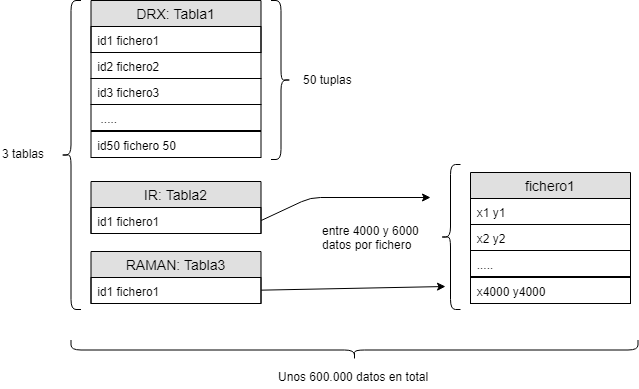
\includegraphics[scale=0.75]{imagenes/disenoBaseDatos/accessDesign.png}
    \caption{Diseño propuesto en Access de la Base de Datos}
    \label{fig:accessDesign}
\end{figure}

En el diseño que yo he propuesto (\textbf{Figura \ref{fig:sqliteDesign}}) lo que tenemos son 3 tablas, cada una de 200.000 entradas (50 x 4000 en el peor de los casos) donde tenemos disponibles todos y cada uno de los datos. Además una de las ventajas de esta forma es que la aplicación no tiene que hacer tantas operaciones de entrada salida para procesar todos los datos al realizar las consultas. Con el diseño propuesto solo se procesan una única vez para poder cargar y generar la base de datos. 

\begin{figure}[H]
    \centering
    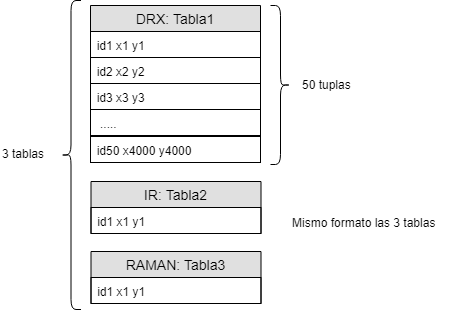
\includegraphics[scale=0.75]{imagenes/disenoBaseDatos/sqliteDesign.png}
    \caption{Diseño propio de la base de datos}
    \label{fig:sqliteDesign}
\end{figure}


\subsubsection{Código frente a eficacia}

Otro de los problemas es la eficacia y el diseño frente a la limpieza y entendibilidad del código. Podemos implementar la solución de dos maneras diferentes. 

La primera es creando una única base de datos con todas las tablas y todas las operaciones necesarias. El problema es que esa base de datos y las operaciones se tienen que crear en una única clase que se encarga de ello, esta clase va a ser relativamente grande y uno de los principios de diseño que por ejemplo podemos encontrar en el Libro Clean Code \cite{cleanCode} es que las clases tienen que ser pequeñas, autocontenidas y hacer una única cosa. Sin embargo nuestra clase va a crear una base de datos, inicializar 4 tablas y ofrecer todos los métodos de acceso y modificación de todas las tablas.

De esta forma el código se ve afectado pero sin embargo el diseño de la base de datos y la eficacia de las consultas no se ve afectada.

La otra manera es crear una clase para cada una de las tablas, pero de esta manera tendríamos una base de datos por tabla, lo que no concuerda con el diseño propuesto de la base de datos y además tendríamos que procesar las consultas via software usando la JVM lo cual puede traducirse en un decremento de la eficiencia de la aplicación. 

La solución por la que se ha optado es la primera. 
 \newpage
\section{Diseño de la base de datos}
\setlength{\parskip}{0.5cm}

En esta sección vamos a mostrar como se ha llevado a cabo el diseño de la base de datos y los diferentes procedimientos utilizados. 

Tenemos que destacar que contamos con una implementación de la base de datos de pigmentos. El problema es que dicha base de datos esta implementada en AccessDB, que es un sistema gestor de bases de datos propietario de Microsoft. Existen herramientas que permiten la integración de dichos tipos de bases de datos en otros gestores como MySQL o SQLite.

En este caso la base de datos se va a diseñar desde 0 para una mejor optimización de los recursos, además se utilizará como sistema gestor de bases de datos SQLite, ya que tiene una integración completa de serie con los terminales Android.

\subsection{Suposiciones y convenciones}
En este apartado se van a aclarar ciertas cosas acerca de los identificadores de las relaciones, formatos que hemos decidido usar y algunas otras convenciones que me parece apropiado comentar en relación al diseño de la base de datos. 

\begin{itemize}
    \item Los identificadores tanto de los pigmentos, que actúan como clave primaria de la mayoría de las relaciones quedan representados por el descriptor breve. En este caso el descriptor es un código numérico que se ira generando de manera automática en la base de datos. De esta forma nos aseguramos de que cada uno de los pigmentos y de los datos relacionados están representados de manera unívoca por un número identificativo. 
    \item Cabe destacar que en el diagrama de entidad relación el formato que se ha seguido para representar las cardinalidades de las relaciones queda representado por el formato típico de UML, y no el que dicta el diseño propio de las bases de datos convencionales. 
\end{itemize}

\subsection{Posibles consultas contra la BBDD}
Vamos a analizar de manera breve las diferentes consultas que podemos realizar contra la base de datos que tenemos que diseñar. En nuestro caso, las consultas quedan determinadas por las diferentes interfaces que vamos a tener en nuestra aplicación. En este caso la principal información que vamos a tener que extraer de la base de datos es la siguiente:

\begin{itemize}
    \item Información acerca de cada uno de los pigmentos: en nuestra aplicación tenemos una vista en la que se muestra una lista con todos los pigmentos junto con la información más básica de cada uno de ellos, como puede ser el nombre, el color y el elemento químico principal por el que están compuestos. Esta información la podemos extraer directamente de la relación Pigmentos, donde tenemos toda la información básica de todos ellos. 
    \item Coordenadas colorimétricas: cada uno de los pigmentos consta de una serie de coordenadas que determinan el color y la luminosidad del mismo. Estas coordenadas serán almacenadas en una relación diferente porque la considero una característica un poco más avanzada que por ejemplo el nombre del pigmento. Cada uno de los pigmentos tendrá una relación directa con sus coordenadas colirimétricas. Esta relación será posible gracias al identificador único del pigmento que será utilizado como clave primaria en todas las relaciones. 
    \item Difractograma de rayos X: cada uno de los pigmentos tiene información relacionada con su generación del difractograma de rayos X característico. Por ello esta información se ha almacenado en una tabla diferente y el método de acceso será equivalente al mencionado en la relación anterior. Tenemos que ser capaces de extraer una gráfica para poder mostrar el espectro de rayos X de cada uno de los elementos que tenemos en la base de datos. 
    \item Infrarojos: otra de las características representativa de cada uno de los pigmentos es su \textcolor{red}{mirar en la documentación las definiciones exactas de cada una de las cosas que estoy poniendo} espectro de infrarojos, básicamente va a estar compuesto por dos valores a partir de los cuales se podrán generar una serie de gráficas. Tenemos que ser capaces de extraer las gráficas correspondientes al espectro de infrarojos para cada uno de los pigmentos.
    \item Espectro de Raman: cada uno de los pigmentos tiene asociado un espectro de Raman característico. Este espectro se puede generar gracias a dos valores, ya que es una gráfica simple, en la que luego tenemos que dar los puntos más representativos. Tenemos que ser capaces de extraer los 3 picos de Raman más importantes junto con las gráficas correspondientes. 
\end{itemize}

\subsection{Modelado conceptual}
\subsubsection{Entidades y atributos}

Las diferentes entidades junto con sus atributos son las siguientes: \textcolor{red}{mirar la definición de cada uno de los atributos de las entidades, además de mirar bien las relaciones}
\begin{itemize}
    \item \textbf{Pigmento}: tenemos que almacenar de una manera segura y persistente la información relacionada con cada uno de los pigmentos. Para ello simplemente vamos a exportar dichos datos de las bases de datos ya existentes y creadas en AccessDB. La información que tenemos que almacenar de cada uno de los pigmentos es la siguiente:
        \begin{itemize}
            \item \textit{Nombre}: nombre con el que se identifica a cada uno de los pigmentos dentro de la base de datos. Dicho nombre es único para cada uno de los pigmentos.
            \item \textit{Id Color}: id representando el color principal de cada uno de los pigmentos
            \item \textit{Notas}: los pigmentos pueden o no tener notas adjuntas, de hecho se permite a los usuarios añadir notas sobre dichos pigmentos. Es por ello que se permiten almacenar notas separadas de cada uno de los elementos de la base de datos.
            \item \textit{Potencia}: \textcolor{red}{TODO}
            \item \textit{Lambda}: \textcolor{red}{TODO}
            \item \textit{Fórmula}: los pigmentos al estar compuestos por elementos naturales, tienen fórmulas químicas determinadas. Es un dato importante si queremos saber su composición o como van a reaccionar cuando están en presencia de cierto elementos químicos, también la mostraremos.
            \item \textit{Sinónimos}: los pigmentos pueden tener sinónimos a la hora de ser llamados. Es por esto que cada uno de ellos tendrá una relación con sus sinónimos. 
            \item \textit{Elemento químico}: cada uno de los pigmentos tiene un elemento químico predominante en su composición química. Tenemos que almacenarlo para mostrarlo cuando proporcionemos la información relacionada con el pigmento.
        \end{itemize}
        
    \item \textbf{Colorimetría}:
        \begin{itemize}
            \item \textit{L}: \textcolor{red}{TODO}
            \item \textit{a}: \textcolor{red}{TODO}
            \item \textit{b}: \textcolor{red}{TODO}
            \item \textit{X}: \textcolor{red}{TODO}
            \item \textit{Y}: \textcolor{red}{TODO}
            \item \textit{Z}: \textcolor{red}{TODO}
            \item \textit{\textcolor{red}{TODO}}: \textcolor{red}{TODO}
        \end{itemize}
        
    \item \textbf{Difractograma de rayos X}:
        \begin{itemize}
            \item \textit{x}: \textcolor{red}{TODO}
            \item \textit{y}: \textcolor{red}{TODO}
        \end{itemize}
        
    \item \textbf{Espectro de Raman}:
        \begin{itemize}
            \item \textit{x}: \textcolor{red}{TODO}
            \item \textit{y}: \textcolor{red}{TODO}
        \end{itemize}
        
    \item \textbf{Espectro de infrarrojos}:
        \begin{itemize}
            \item \textit{x}: \textcolor{red}{TODO}
            \item \textit{y}: \textcolor{red}{TODO}
        \end{itemize}
        
    \item \textbf{Notas}: el usuario tiene que ser capaz de escribir notas rápidas para sí mismo acerca de cada uno de los pigmentos. Es por ello que una de las opciones de la aplicación es almacenar notas de uno de los pigmentos seleccionados. Dichas notas podrán ser recuperadas con posterioridad por el usuario para ser editadas o borradas.
        \begin{itemize}
            \item \textit{Título}: cada una de las notas que almacenamos de un pigmento consta de un título, que no es único y va a tener una longitud limitada a 100 caracteres. Tiene que ser algo corto y determinado. Ya que lo primero que ser verá cuando mostremos la vista de las notas es el título y estarán ordenadas por la fecha de creación, por lo que la última nota creada es la que se mostrará por completo. 
            \item \textit{Valor}: el valor es la nota en sí. Lo que el usuario introduzca en el formulario de escritura. 
            \item \textit{Fecha}: la fecha no será necesario mostrarla al usuario, pero si que tiene sentido almacenarla en la base da datos para tener un histórico de creación de las mismas y luego poder recuperarlas en diferente orden por la aplicación.  
        \end{itemize}
        
    \item \textbf{Sinónimos}: cada uno de los pigmentos puede tener nombres diferentes con los que ha sido referenciado a lo largo del tiempo. Es por esto que tendremos un lista para cada uno de los pigmentos con todos los sinónimos que tenga. 
        \begin{itemize}
            \item \textit{Valor}: como cada uno de los sinónimos puede tener 0 o más sinónimos, he decidido hacer una relación separada para cada uno de los pigmentos. Sino otra forma es hacer un atributo sinónimo dentro de la entidad Pigmento conteniendo una lista separada por comas con todos los sinónimos, pero me parece una mejor opción hacer una relación separada. 
        \end{itemize}
\end{itemize}

Antes de mostrar el diagrama de entidad relación vamos a mostrar una pequeña tabla con las diferentes cardinalidades y entidades relacionadas. Podemos encontrar dicho gráfico en la \textbf{Figura \ref{fig:cardinalidades}}

\begin{figure}[H]
    \centering
    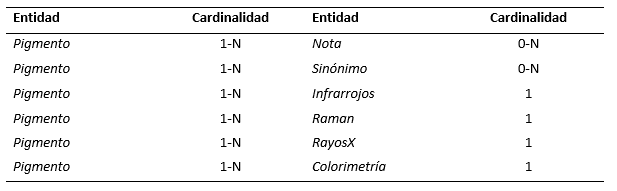
\includegraphics[scale=1]{imagenes/disenoBaseDatos/cardinalidades.png}
    \caption{Entidades y cardinalidades del modelo}
    \label{fig:cardinalidades}
\end{figure}

\subsubsection{Diagrama de Entidad Relación}

Una vez que hemos presentado tanto las entidades, como las cardinalidades y como están relacionadas las mismas, podemos mostrar como se relacionan las unas con las otras de una manera gráfica, que es presentado el diagrama de entidad relación de la base de datos. En este caso se ha decidido usar el formato de UML y no sigue las reglas estrictas del modelo de Entidad Relación, pero me parece que es más visual, la herramienta y el formato es más universal y entendible que el propio para expresar este tipo de contenidos. Podemos encontrar esto en la \textbf{Figura \ref{fig:diagramaER}}

\begin{figure}[H]
    \centering
    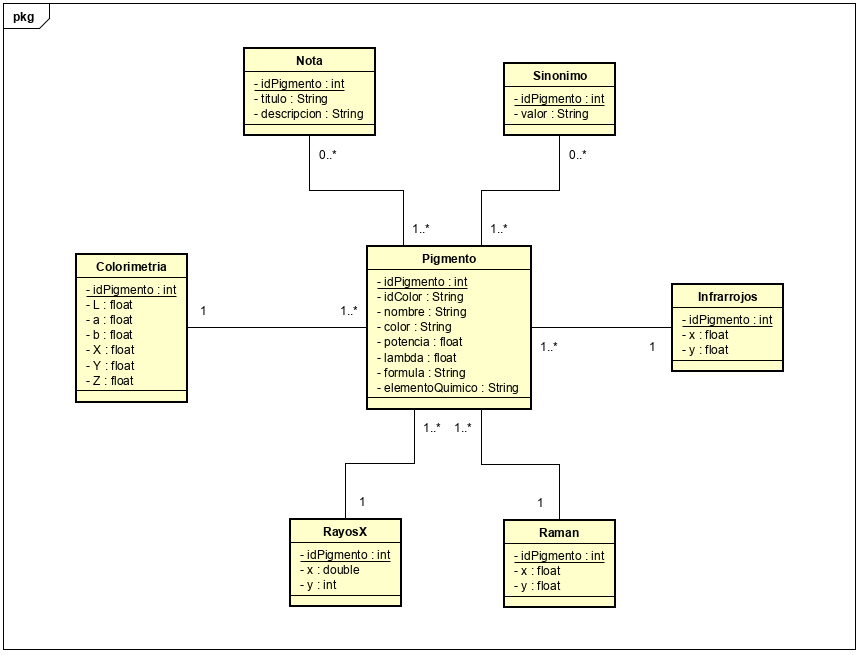
\includegraphics[scale=0.75]{imagenes/disenoBaseDatos/diagramaER.png}
    \caption{Diagrama de Entidad-Relación de la base de datos}
    \label{fig:diagramaER}
\end{figure}

En el diagrama podemos observar como la clave primaria de todas las relaciones es el id del pigmento en cuestión. Esto luego nos permitirá conectar unas relaciones con otras y buscar la información de una manera más adecuada. 

\textcolor{red}{mirar a ver las transformaciones y buscar un poco mas de teoría de diseño de la base de datos}

Una vez que tenemos el diseño de la base de datos podemos pasar a explicar la implementación de la misma, en lineas generales. 


\subsection{Implementación de la base de datos}
Una vez que tenemos la base de datos diseñada tenemos que implementarla dentro de nuestra aplicación. Para ello lo primero que tenemos que hacer es crear una clase auxiliar que nos permita la creación y en el futuro la conexión entre la propia aplicación y los datos almacenados en la base de datos. 

Para implementar la base de datos he optado por hacerlo de una manera más sencilla que la aprendida en la asignatura de SMOV. La base en realidad es la misma, pero la forma es la misma, bien es sabido que dentro de la informática podemos obtener los mismos resultados pero con algoritmos diferentes. En este caso vamos a realizar una mezcla entre uno de los patrones de acceso comentados al principio, DAO y los POJO.

Como hemos dicho en los capítulos anteriores, cada uno de los elementos de la base de datos, que en este caso son pigmentos, va a estar representado por un objeto típico de Java. Esta forma de representar los objetos para el almacenamiento de datos se denomina POJO (\textbf{P}lain \textbf{O}ld \textbf{J}ava \textbf{O}bjects).

Además cada vez que recuperemos los elementos de la base de datos lo hacemos devolviendo una lista de objetos del tipo adecuado. Por ejemplo para devolver todos y cada uno de los pigmentos que hay en la base de datos lo que hacemos es mandar la consulta al SGBD de SQLite y lo que nos devuelve es una lista de POJOs del tipo deseado. 

De esta manera podemos acceder de una manera sencilla a todos los atributos de los datos que acabamos de recuperar.

\subsubsection{¿Que son los POJO?} 

Dicho término \cite{pojo} fue acuñado por Martin Fowler, Rebecca Parsons y Josh MacKenzie en Septiembre del 2000. Se usa para referirse a un objeto Java que no tiene limitaciones de por requerir librerías ni clases externas. Son objetos simples y básicos de java, con atributos, funciones para recuperar los valores y para cambiarlos en caso necesario y nada más. Este tipo de objetos son muy utilizados cuando tenemos que convertir objetos entre diferentes lenguajes o cuando tenemos que serializarlos para enviarlos por la red. 

Idealmente y según dice la definición de los mismos, un objeto Java es POJO si cumple estos 3 requisitos:
\begin{itemize}
    \item No extiende de ninguna clase. 
        \begin{figure}[H]
        \lstinputlisting[style=customc]{capitulos/disenoBaseDatos/codigo/noExtiende.java}
        \label{fig:noExtiende}
        \end{figure}
    
    \item No implementa ninguna clase. 
        \begin{figure}[H]
        \lstinputlisting[style=customc]{capitulos/disenoBaseDatos/codigo/noImplementa.java}
        \label{fig:noImplementa}
        \end{figure}
        
    \item No contiene anotaciones. 
        \begin{figure}[H] 
        \lstinputlisting[style=customc]{capitulos/disenoBaseDatos/codigo/noAnotaciones.java}
        \label{fig:noAnotaciones}
        \end{figure}
\end{itemize}

Los POJO fueron inicialmente utilizados en J2EE para representar los JavaBeans, que son objetos java muy simples y que ofrecen servicios por la red. Se siguen utilizando aunque han cambiado un poco las formas de hacerlo. Ahora los POJO también son ampliamente utilizados para representar objetos JSON recibidos por parte de microservicios web y ser utilizados en un servidor. Este es uno de los muchos ejemplos de utilización real a día de hoy de los POJO. 

\subsubsection{Ejemplo}

Vamos a explicar con un sencillo ejemplo lo que son los POJO y como se hace la consulta de los mismos para luego mostrar la información dentro de la aplicación.

En este caso uno de los atributos que nos interesa son las diferentes notas que tiene cada uno de los pigmentos, para ello habrá una tabla con todas las notas de todos los pigmentos. Como hemos enseñado en el modelado conceptual, de cada una de las diferentes notas almacenamos y guardamos los siguientes datos: 
\begin{itemize}
    \item IdPigmento: para poder relacionar la nota con el pigmento, este dato es interno para la gestión de los datos. 
    \item Título: breve descripción.
    \item Descripción: contenido completo de la nota. 
    \item Fecha: fecha de creación de la misma. 
\end{itemize}

La descripción anterior la podemos encontrar representada por un POJO en el siguiente fragmento de cñodigo Java: 

\begin{figure}[H] 
\lstinputlisting[style=customc]{capitulos/disenoBaseDatos/codigo/notaPojo.java}
\label{fig:notaPojo}
\end{figure}





\subsection{Otras consideraciones}
Algunas otras decisiones de diseño que hemos tenido que tener en cuenta, y que afectan tanto al rendimiento de la aplicación como al diseño de la base de datos, son las siguientes:

\subsubsection{Diseño antiguo VS diseño actual}
En el diseño antiguo de la base de datos (\textbf{Figura \ref{fig:accessDesign}}), de manera resumida se tiene una tabla con una entrada para cada pigmento y esta entrada tiene un atributo que referencia a un fichero de datos. Por ejemplo si queremos obtener el difractograma de rayos X del pigmento número 3, nos va a referenciar a un fichero de texto que contiene aproximadamente unas 4000 líneas con 2 valores en cada línea. Es decir que en total vamos a tener unos 50 ficheros cada uno de 4000 líneas. Según el gestor de almacenamiento de Windows estos ficheros tienen un tamaño medio de unos 30 Kb. En total tenemos unos 150 ficheros lo que hace que el total de los ficheros si los tuviéramos que almacenar dentro de la base de datos para su posterior procesado, además de tener aparte la instancia de la base de datos creada supondría un aumento de unos 5Mb en la aplicación.

\begin{figure}[H]
    \centering
    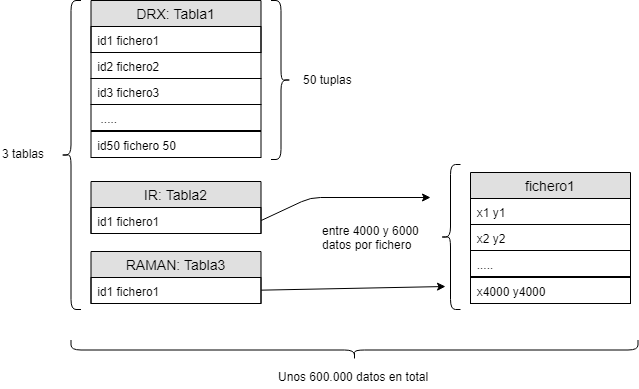
\includegraphics[scale=0.75]{imagenes/disenoBaseDatos/accessDesign.png}
    \caption{Diseño propuesto en Access de la Base de Datos}
    \label{fig:accessDesign}
\end{figure}

En el diseño que yo he propuesto (\textbf{Figura \ref{fig:sqliteDesign}}) lo que tenemos son 3 tablas, cada una de 200.000 entradas (50 x 4000 en el peor de los casos) donde tenemos disponibles todos y cada uno de los datos. Además una de las ventajas de esta forma es que la aplicación no tiene que hacer tantas operaciones de entrada salida para procesar todos los datos al realizar las consultas. Con el diseño propuesto solo se procesan una única vez para poder cargar y generar la base de datos. 

\begin{figure}[H]
    \centering
    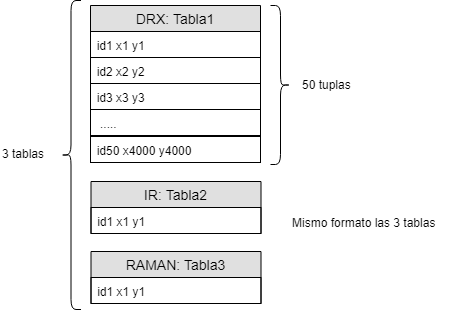
\includegraphics[scale=0.75]{imagenes/disenoBaseDatos/sqliteDesign.png}
    \caption{Diseño propio de la base de datos}
    \label{fig:sqliteDesign}
\end{figure}


\subsubsection{Código frente a eficacia}

Otro de los problemas es la eficacia y el diseño frente a la limpieza y entendibilidad del código. Podemos implementar la solución de dos maneras diferentes. 

La primera es creando una única base de datos con todas las tablas y todas las operaciones necesarias. El problema es que esa base de datos y las operaciones se tienen que crear en una única clase que se encarga de ello, esta clase va a ser relativamente grande y uno de los principios de diseño que por ejemplo podemos encontrar en el Libro Clean Code \cite{cleanCode} es que las clases tienen que ser pequeñas, autocontenidas y hacer una única cosa. Sin embargo nuestra clase va a crear una base de datos, inicializar 4 tablas y ofrecer todos los métodos de acceso y modificación de todas las tablas.

De esta forma el código se ve afectado pero sin embargo el diseño de la base de datos y la eficacia de las consultas no se ve afectada.

La otra manera es crear una clase para cada una de las tablas, pero de esta manera tendríamos una base de datos por tabla, lo que no concuerda con el diseño propuesto de la base de datos y además tendríamos que procesar las consultas via software usando la JVM lo cual puede traducirse en un decremento de la eficiencia de la aplicación. 

La solución por la que se ha optado es la primera. 
 \newpage
\section{Diseño de la base de datos}
\setlength{\parskip}{0.5cm}

En esta sección vamos a mostrar como se ha llevado a cabo el diseño de la base de datos y los diferentes procedimientos utilizados. 

Tenemos que destacar que contamos con una implementación de la base de datos de pigmentos. El problema es que dicha base de datos esta implementada en AccessDB, que es un sistema gestor de bases de datos propietario de Microsoft. Existen herramientas que permiten la integración de dichos tipos de bases de datos en otros gestores como MySQL o SQLite.

En este caso la base de datos se va a diseñar desde 0 para una mejor optimización de los recursos, además se utilizará como sistema gestor de bases de datos SQLite, ya que tiene una integración completa de serie con los terminales Android.

\subsection{Suposiciones y convenciones}
En este apartado se van a aclarar ciertas cosas acerca de los identificadores de las relaciones, formatos que hemos decidido usar y algunas otras convenciones que me parece apropiado comentar en relación al diseño de la base de datos. 

\begin{itemize}
    \item Los identificadores tanto de los pigmentos, que actúan como clave primaria de la mayoría de las relaciones quedan representados por el descriptor breve. En este caso el descriptor es un código numérico que se ira generando de manera automática en la base de datos. De esta forma nos aseguramos de que cada uno de los pigmentos y de los datos relacionados están representados de manera unívoca por un número identificativo. 
    \item Cabe destacar que en el diagrama de entidad relación el formato que se ha seguido para representar las cardinalidades de las relaciones queda representado por el formato típico de UML, y no el que dicta el diseño propio de las bases de datos convencionales. 
\end{itemize}

\subsection{Posibles consultas contra la BBDD}
Vamos a analizar de manera breve las diferentes consultas que podemos realizar contra la base de datos que tenemos que diseñar. En nuestro caso, las consultas quedan determinadas por las diferentes interfaces que vamos a tener en nuestra aplicación. En este caso la principal información que vamos a tener que extraer de la base de datos es la siguiente:

\begin{itemize}
    \item Información acerca de cada uno de los pigmentos: en nuestra aplicación tenemos una vista en la que se muestra una lista con todos los pigmentos junto con la información más básica de cada uno de ellos, como puede ser el nombre, el color y el elemento químico principal por el que están compuestos. Esta información la podemos extraer directamente de la relación Pigmentos, donde tenemos toda la información básica de todos ellos. 
    \item Coordenadas colorimétricas: cada uno de los pigmentos consta de una serie de coordenadas que determinan el color y la luminosidad del mismo. Estas coordenadas serán almacenadas en una relación diferente porque la considero una característica un poco más avanzada que por ejemplo el nombre del pigmento. Cada uno de los pigmentos tendrá una relación directa con sus coordenadas colirimétricas. Esta relación será posible gracias al identificador único del pigmento que será utilizado como clave primaria en todas las relaciones. 
    \item Difractograma de rayos X: cada uno de los pigmentos tiene información relacionada con su generación del difractograma de rayos X característico. Por ello esta información se ha almacenado en una tabla diferente y el método de acceso será equivalente al mencionado en la relación anterior. Tenemos que ser capaces de extraer una gráfica para poder mostrar el espectro de rayos X de cada uno de los elementos que tenemos en la base de datos. 
    \item Infrarojos: otra de las características representativa de cada uno de los pigmentos es su \textcolor{red}{mirar en la documentación las definiciones exactas de cada una de las cosas que estoy poniendo} espectro de infrarojos, básicamente va a estar compuesto por dos valores a partir de los cuales se podrán generar una serie de gráficas. Tenemos que ser capaces de extraer las gráficas correspondientes al espectro de infrarojos para cada uno de los pigmentos.
    \item Espectro de Raman: cada uno de los pigmentos tiene asociado un espectro de Raman característico. Este espectro se puede generar gracias a dos valores, ya que es una gráfica simple, en la que luego tenemos que dar los puntos más representativos. Tenemos que ser capaces de extraer los 3 picos de Raman más importantes junto con las gráficas correspondientes. 
\end{itemize}

\subsection{Modelado conceptual}
\subsubsection{Entidades y atributos}

Las diferentes entidades junto con sus atributos son las siguientes: \textcolor{red}{mirar la definición de cada uno de los atributos de las entidades, además de mirar bien las relaciones}
\begin{itemize}
    \item \textbf{Pigmento}: tenemos que almacenar de una manera segura y persistente la información relacionada con cada uno de los pigmentos. Para ello simplemente vamos a exportar dichos datos de las bases de datos ya existentes y creadas en AccessDB. La información que tenemos que almacenar de cada uno de los pigmentos es la siguiente:
        \begin{itemize}
            \item \textit{Nombre}: nombre con el que se identifica a cada uno de los pigmentos dentro de la base de datos. Dicho nombre es único para cada uno de los pigmentos.
            \item \textit{Id Color}: id representando el color principal de cada uno de los pigmentos
            \item \textit{Notas}: los pigmentos pueden o no tener notas adjuntas, de hecho se permite a los usuarios añadir notas sobre dichos pigmentos. Es por ello que se permiten almacenar notas separadas de cada uno de los elementos de la base de datos.
            \item \textit{Potencia}: \textcolor{red}{TODO}
            \item \textit{Lambda}: \textcolor{red}{TODO}
            \item \textit{Fórmula}: los pigmentos al estar compuestos por elementos naturales, tienen fórmulas químicas determinadas. Es un dato importante si queremos saber su composición o como van a reaccionar cuando están en presencia de cierto elementos químicos, también la mostraremos.
            \item \textit{Sinónimos}: los pigmentos pueden tener sinónimos a la hora de ser llamados. Es por esto que cada uno de ellos tendrá una relación con sus sinónimos. 
            \item \textit{Elemento químico}: cada uno de los pigmentos tiene un elemento químico predominante en su composición química. Tenemos que almacenarlo para mostrarlo cuando proporcionemos la información relacionada con el pigmento.
        \end{itemize}
        
    \item \textbf{Colorimetría}:
        \begin{itemize}
            \item \textit{L}: \textcolor{red}{TODO}
            \item \textit{a}: \textcolor{red}{TODO}
            \item \textit{b}: \textcolor{red}{TODO}
            \item \textit{X}: \textcolor{red}{TODO}
            \item \textit{Y}: \textcolor{red}{TODO}
            \item \textit{Z}: \textcolor{red}{TODO}
            \item \textit{\textcolor{red}{TODO}}: \textcolor{red}{TODO}
        \end{itemize}
        
    \item \textbf{Difractograma de rayos X}:
        \begin{itemize}
            \item \textit{x}: \textcolor{red}{TODO}
            \item \textit{y}: \textcolor{red}{TODO}
        \end{itemize}
        
    \item \textbf{Espectro de Raman}:
        \begin{itemize}
            \item \textit{x}: \textcolor{red}{TODO}
            \item \textit{y}: \textcolor{red}{TODO}
        \end{itemize}
        
    \item \textbf{Espectro de infrarrojos}:
        \begin{itemize}
            \item \textit{x}: \textcolor{red}{TODO}
            \item \textit{y}: \textcolor{red}{TODO}
        \end{itemize}
        
    \item \textbf{Notas}: el usuario tiene que ser capaz de escribir notas rápidas para sí mismo acerca de cada uno de los pigmentos. Es por ello que una de las opciones de la aplicación es almacenar notas de uno de los pigmentos seleccionados. Dichas notas podrán ser recuperadas con posterioridad por el usuario para ser editadas o borradas.
        \begin{itemize}
            \item \textit{Título}: cada una de las notas que almacenamos de un pigmento consta de un título, que no es único y va a tener una longitud limitada a 100 caracteres. Tiene que ser algo corto y determinado. Ya que lo primero que ser verá cuando mostremos la vista de las notas es el título y estarán ordenadas por la fecha de creación, por lo que la última nota creada es la que se mostrará por completo. 
            \item \textit{Valor}: el valor es la nota en sí. Lo que el usuario introduzca en el formulario de escritura. 
            \item \textit{Fecha}: la fecha no será necesario mostrarla al usuario, pero si que tiene sentido almacenarla en la base da datos para tener un histórico de creación de las mismas y luego poder recuperarlas en diferente orden por la aplicación.  
        \end{itemize}
        
    \item \textbf{Sinónimos}: cada uno de los pigmentos puede tener nombres diferentes con los que ha sido referenciado a lo largo del tiempo. Es por esto que tendremos un lista para cada uno de los pigmentos con todos los sinónimos que tenga. 
        \begin{itemize}
            \item \textit{Valor}: como cada uno de los sinónimos puede tener 0 o más sinónimos, he decidido hacer una relación separada para cada uno de los pigmentos. Sino otra forma es hacer un atributo sinónimo dentro de la entidad Pigmento conteniendo una lista separada por comas con todos los sinónimos, pero me parece una mejor opción hacer una relación separada. 
        \end{itemize}
\end{itemize}

Antes de mostrar el diagrama de entidad relación vamos a mostrar una pequeña tabla con las diferentes cardinalidades y entidades relacionadas. Podemos encontrar dicho gráfico en la \textbf{Figura \ref{fig:cardinalidades}}

\begin{figure}[H]
    \centering
    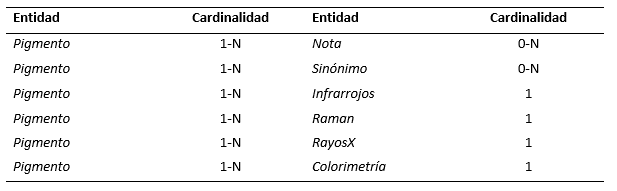
\includegraphics[scale=1]{imagenes/disenoBaseDatos/cardinalidades.png}
    \caption{Entidades y cardinalidades del modelo}
    \label{fig:cardinalidades}
\end{figure}

\subsubsection{Diagrama de Entidad Relación}

Una vez que hemos presentado tanto las entidades, como las cardinalidades y como están relacionadas las mismas, podemos mostrar como se relacionan las unas con las otras de una manera gráfica, que es presentado el diagrama de entidad relación de la base de datos. En este caso se ha decidido usar el formato de UML y no sigue las reglas estrictas del modelo de Entidad Relación, pero me parece que es más visual, la herramienta y el formato es más universal y entendible que el propio para expresar este tipo de contenidos. Podemos encontrar esto en la \textbf{Figura \ref{fig:diagramaER}}

\begin{figure}[H]
    \centering
    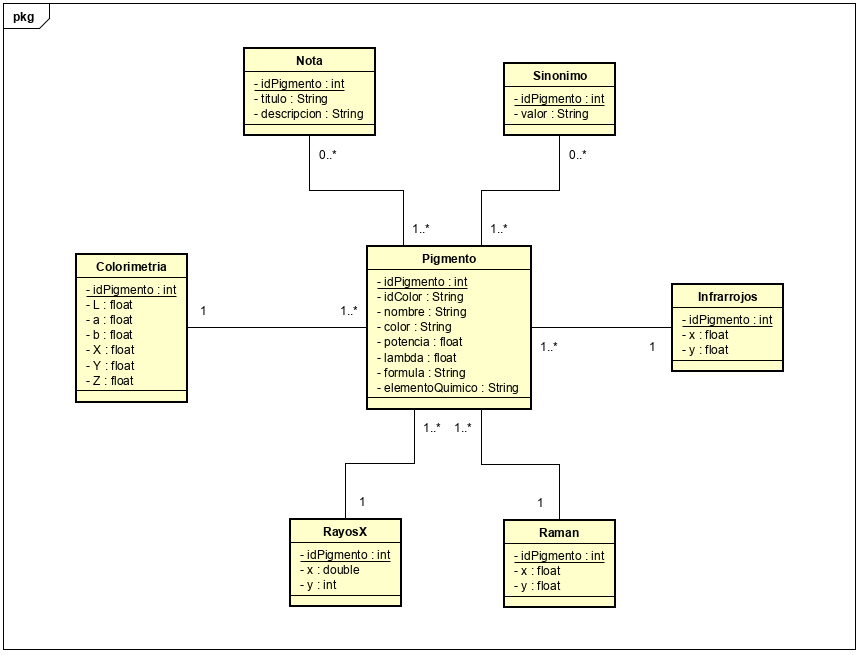
\includegraphics[scale=0.75]{imagenes/disenoBaseDatos/diagramaER.png}
    \caption{Diagrama de Entidad-Relación de la base de datos}
    \label{fig:diagramaER}
\end{figure}

En el diagrama podemos observar como la clave primaria de todas las relaciones es el id del pigmento en cuestión. Esto luego nos permitirá conectar unas relaciones con otras y buscar la información de una manera más adecuada. 

\textcolor{red}{mirar a ver las transformaciones y buscar un poco mas de teoría de diseño de la base de datos}

Una vez que tenemos el diseño de la base de datos podemos pasar a explicar la implementación de la misma, en lineas generales. 


\subsection{Implementación de la base de datos}
Una vez que tenemos la base de datos diseñada tenemos que implementarla dentro de nuestra aplicación. Para ello lo primero que tenemos que hacer es crear una clase auxiliar que nos permita la creación y en el futuro la conexión entre la propia aplicación y los datos almacenados en la base de datos. 

Para implementar la base de datos he optado por hacerlo de una manera más sencilla que la aprendida en la asignatura de SMOV. La base en realidad es la misma, pero la forma es la misma, bien es sabido que dentro de la informática podemos obtener los mismos resultados pero con algoritmos diferentes. En este caso vamos a realizar una mezcla entre uno de los patrones de acceso comentados al principio, DAO y los POJO.

Como hemos dicho en los capítulos anteriores, cada uno de los elementos de la base de datos, que en este caso son pigmentos, va a estar representado por un objeto típico de Java. Esta forma de representar los objetos para el almacenamiento de datos se denomina POJO (\textbf{P}lain \textbf{O}ld \textbf{J}ava \textbf{O}bjects).

Además cada vez que recuperemos los elementos de la base de datos lo hacemos devolviendo una lista de objetos del tipo adecuado. Por ejemplo para devolver todos y cada uno de los pigmentos que hay en la base de datos lo que hacemos es mandar la consulta al SGBD de SQLite y lo que nos devuelve es una lista de POJOs del tipo deseado. 

De esta manera podemos acceder de una manera sencilla a todos los atributos de los datos que acabamos de recuperar.

\subsubsection{¿Que son los POJO?} 

Dicho término \cite{pojo} fue acuñado por Martin Fowler, Rebecca Parsons y Josh MacKenzie en Septiembre del 2000. Se usa para referirse a un objeto Java que no tiene limitaciones de por requerir librerías ni clases externas. Son objetos simples y básicos de java, con atributos, funciones para recuperar los valores y para cambiarlos en caso necesario y nada más. Este tipo de objetos son muy utilizados cuando tenemos que convertir objetos entre diferentes lenguajes o cuando tenemos que serializarlos para enviarlos por la red. 

Idealmente y según dice la definición de los mismos, un objeto Java es POJO si cumple estos 3 requisitos:
\begin{itemize}
    \item No extiende de ninguna clase. 
        \begin{figure}[H]
        \lstinputlisting[style=customc]{capitulos/disenoBaseDatos/codigo/noExtiende.java}
        \label{fig:noExtiende}
        \end{figure}
    
    \item No implementa ninguna clase. 
        \begin{figure}[H]
        \lstinputlisting[style=customc]{capitulos/disenoBaseDatos/codigo/noImplementa.java}
        \label{fig:noImplementa}
        \end{figure}
        
    \item No contiene anotaciones. 
        \begin{figure}[H] 
        \lstinputlisting[style=customc]{capitulos/disenoBaseDatos/codigo/noAnotaciones.java}
        \label{fig:noAnotaciones}
        \end{figure}
\end{itemize}

Los POJO fueron inicialmente utilizados en J2EE para representar los JavaBeans, que son objetos java muy simples y que ofrecen servicios por la red. Se siguen utilizando aunque han cambiado un poco las formas de hacerlo. Ahora los POJO también son ampliamente utilizados para representar objetos JSON recibidos por parte de microservicios web y ser utilizados en un servidor. Este es uno de los muchos ejemplos de utilización real a día de hoy de los POJO. 

\subsubsection{Ejemplo}

Vamos a explicar con un sencillo ejemplo lo que son los POJO y como se hace la consulta de los mismos para luego mostrar la información dentro de la aplicación.

En este caso uno de los atributos que nos interesa son las diferentes notas que tiene cada uno de los pigmentos, para ello habrá una tabla con todas las notas de todos los pigmentos. Como hemos enseñado en el modelado conceptual, de cada una de las diferentes notas almacenamos y guardamos los siguientes datos: 
\begin{itemize}
    \item IdPigmento: para poder relacionar la nota con el pigmento, este dato es interno para la gestión de los datos. 
    \item Título: breve descripción.
    \item Descripción: contenido completo de la nota. 
    \item Fecha: fecha de creación de la misma. 
\end{itemize}

La descripción anterior la podemos encontrar representada por un POJO en el siguiente fragmento de cñodigo Java: 

\begin{figure}[H] 
\lstinputlisting[style=customc]{capitulos/disenoBaseDatos/codigo/notaPojo.java}
\label{fig:notaPojo}
\end{figure}





\subsection{Otras consideraciones}
Algunas otras decisiones de diseño que hemos tenido que tener en cuenta, y que afectan tanto al rendimiento de la aplicación como al diseño de la base de datos, son las siguientes:

\subsubsection{Diseño antiguo VS diseño actual}
En el diseño antiguo de la base de datos (\textbf{Figura \ref{fig:accessDesign}}), de manera resumida se tiene una tabla con una entrada para cada pigmento y esta entrada tiene un atributo que referencia a un fichero de datos. Por ejemplo si queremos obtener el difractograma de rayos X del pigmento número 3, nos va a referenciar a un fichero de texto que contiene aproximadamente unas 4000 líneas con 2 valores en cada línea. Es decir que en total vamos a tener unos 50 ficheros cada uno de 4000 líneas. Según el gestor de almacenamiento de Windows estos ficheros tienen un tamaño medio de unos 30 Kb. En total tenemos unos 150 ficheros lo que hace que el total de los ficheros si los tuviéramos que almacenar dentro de la base de datos para su posterior procesado, además de tener aparte la instancia de la base de datos creada supondría un aumento de unos 5Mb en la aplicación.

\begin{figure}[H]
    \centering
    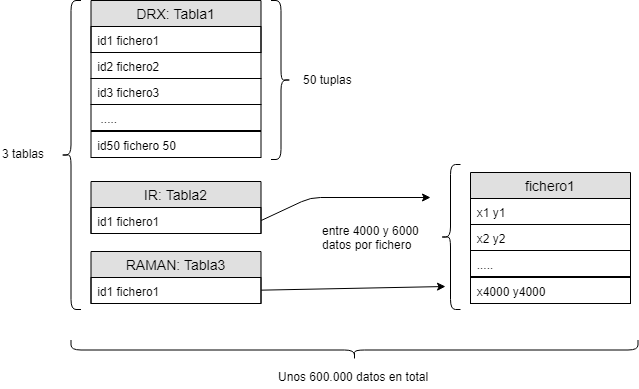
\includegraphics[scale=0.75]{imagenes/disenoBaseDatos/accessDesign.png}
    \caption{Diseño propuesto en Access de la Base de Datos}
    \label{fig:accessDesign}
\end{figure}

En el diseño que yo he propuesto (\textbf{Figura \ref{fig:sqliteDesign}}) lo que tenemos son 3 tablas, cada una de 200.000 entradas (50 x 4000 en el peor de los casos) donde tenemos disponibles todos y cada uno de los datos. Además una de las ventajas de esta forma es que la aplicación no tiene que hacer tantas operaciones de entrada salida para procesar todos los datos al realizar las consultas. Con el diseño propuesto solo se procesan una única vez para poder cargar y generar la base de datos. 

\begin{figure}[H]
    \centering
    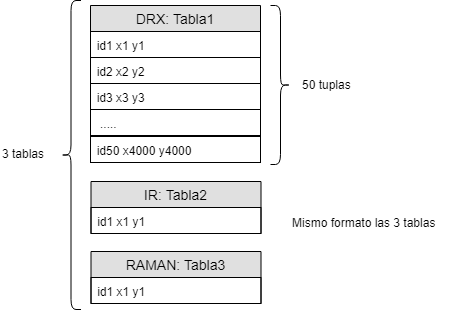
\includegraphics[scale=0.75]{imagenes/disenoBaseDatos/sqliteDesign.png}
    \caption{Diseño propio de la base de datos}
    \label{fig:sqliteDesign}
\end{figure}


\subsubsection{Código frente a eficacia}

Otro de los problemas es la eficacia y el diseño frente a la limpieza y entendibilidad del código. Podemos implementar la solución de dos maneras diferentes. 

La primera es creando una única base de datos con todas las tablas y todas las operaciones necesarias. El problema es que esa base de datos y las operaciones se tienen que crear en una única clase que se encarga de ello, esta clase va a ser relativamente grande y uno de los principios de diseño que por ejemplo podemos encontrar en el Libro Clean Code \cite{cleanCode} es que las clases tienen que ser pequeñas, autocontenidas y hacer una única cosa. Sin embargo nuestra clase va a crear una base de datos, inicializar 4 tablas y ofrecer todos los métodos de acceso y modificación de todas las tablas.

De esta forma el código se ve afectado pero sin embargo el diseño de la base de datos y la eficacia de las consultas no se ve afectada.

La otra manera es crear una clase para cada una de las tablas, pero de esta manera tendríamos una base de datos por tabla, lo que no concuerda con el diseño propuesto de la base de datos y además tendríamos que procesar las consultas via software usando la JVM lo cual puede traducirse en un decremento de la eficiencia de la aplicación. 

La solución por la que se ha optado es la primera. 
 \newpage
\section{Diseño de la base de datos}
\setlength{\parskip}{0.5cm}

En esta sección vamos a mostrar como se ha llevado a cabo el diseño de la base de datos y los diferentes procedimientos utilizados. 

Tenemos que destacar que contamos con una implementación de la base de datos de pigmentos. El problema es que dicha base de datos esta implementada en AccessDB, que es un sistema gestor de bases de datos propietario de Microsoft. Existen herramientas que permiten la integración de dichos tipos de bases de datos en otros gestores como MySQL o SQLite.

En este caso la base de datos se va a diseñar desde 0 para una mejor optimización de los recursos, además se utilizará como sistema gestor de bases de datos SQLite, ya que tiene una integración completa de serie con los terminales Android.

\subsection{Suposiciones y convenciones}
En este apartado se van a aclarar ciertas cosas acerca de los identificadores de las relaciones, formatos que hemos decidido usar y algunas otras convenciones que me parece apropiado comentar en relación al diseño de la base de datos. 

\begin{itemize}
    \item Los identificadores tanto de los pigmentos, que actúan como clave primaria de la mayoría de las relaciones quedan representados por el descriptor breve. En este caso el descriptor es un código numérico que se ira generando de manera automática en la base de datos. De esta forma nos aseguramos de que cada uno de los pigmentos y de los datos relacionados están representados de manera unívoca por un número identificativo. 
    \item Cabe destacar que en el diagrama de entidad relación el formato que se ha seguido para representar las cardinalidades de las relaciones queda representado por el formato típico de UML, y no el que dicta el diseño propio de las bases de datos convencionales. 
\end{itemize}

\subsection{Posibles consultas contra la BBDD}
Vamos a analizar de manera breve las diferentes consultas que podemos realizar contra la base de datos que tenemos que diseñar. En nuestro caso, las consultas quedan determinadas por las diferentes interfaces que vamos a tener en nuestra aplicación. En este caso la principal información que vamos a tener que extraer de la base de datos es la siguiente:

\begin{itemize}
    \item Información acerca de cada uno de los pigmentos: en nuestra aplicación tenemos una vista en la que se muestra una lista con todos los pigmentos junto con la información más básica de cada uno de ellos, como puede ser el nombre, el color y el elemento químico principal por el que están compuestos. Esta información la podemos extraer directamente de la relación Pigmentos, donde tenemos toda la información básica de todos ellos. 
    \item Coordenadas colorimétricas: cada uno de los pigmentos consta de una serie de coordenadas que determinan el color y la luminosidad del mismo. Estas coordenadas serán almacenadas en una relación diferente porque la considero una característica un poco más avanzada que por ejemplo el nombre del pigmento. Cada uno de los pigmentos tendrá una relación directa con sus coordenadas colirimétricas. Esta relación será posible gracias al identificador único del pigmento que será utilizado como clave primaria en todas las relaciones. 
    \item Difractograma de rayos X: cada uno de los pigmentos tiene información relacionada con su generación del difractograma de rayos X característico. Por ello esta información se ha almacenado en una tabla diferente y el método de acceso será equivalente al mencionado en la relación anterior. Tenemos que ser capaces de extraer una gráfica para poder mostrar el espectro de rayos X de cada uno de los elementos que tenemos en la base de datos. 
    \item Infrarojos: otra de las características representativa de cada uno de los pigmentos es su \textcolor{red}{mirar en la documentación las definiciones exactas de cada una de las cosas que estoy poniendo} espectro de infrarojos, básicamente va a estar compuesto por dos valores a partir de los cuales se podrán generar una serie de gráficas. Tenemos que ser capaces de extraer las gráficas correspondientes al espectro de infrarojos para cada uno de los pigmentos.
    \item Espectro de Raman: cada uno de los pigmentos tiene asociado un espectro de Raman característico. Este espectro se puede generar gracias a dos valores, ya que es una gráfica simple, en la que luego tenemos que dar los puntos más representativos. Tenemos que ser capaces de extraer los 3 picos de Raman más importantes junto con las gráficas correspondientes. 
\end{itemize}

\subsection{Modelado conceptual}
\subsubsection{Entidades y atributos}

Las diferentes entidades junto con sus atributos son las siguientes: \textcolor{red}{mirar la definición de cada uno de los atributos de las entidades, además de mirar bien las relaciones}
\begin{itemize}
    \item \textbf{Pigmento}: tenemos que almacenar de una manera segura y persistente la información relacionada con cada uno de los pigmentos. Para ello simplemente vamos a exportar dichos datos de las bases de datos ya existentes y creadas en AccessDB. La información que tenemos que almacenar de cada uno de los pigmentos es la siguiente:
        \begin{itemize}
            \item \textit{Nombre}: nombre con el que se identifica a cada uno de los pigmentos dentro de la base de datos. Dicho nombre es único para cada uno de los pigmentos.
            \item \textit{Id Color}: id representando el color principal de cada uno de los pigmentos
            \item \textit{Notas}: los pigmentos pueden o no tener notas adjuntas, de hecho se permite a los usuarios añadir notas sobre dichos pigmentos. Es por ello que se permiten almacenar notas separadas de cada uno de los elementos de la base de datos.
            \item \textit{Potencia}: \textcolor{red}{TODO}
            \item \textit{Lambda}: \textcolor{red}{TODO}
            \item \textit{Fórmula}: los pigmentos al estar compuestos por elementos naturales, tienen fórmulas químicas determinadas. Es un dato importante si queremos saber su composición o como van a reaccionar cuando están en presencia de cierto elementos químicos, también la mostraremos.
            \item \textit{Sinónimos}: los pigmentos pueden tener sinónimos a la hora de ser llamados. Es por esto que cada uno de ellos tendrá una relación con sus sinónimos. 
            \item \textit{Elemento químico}: cada uno de los pigmentos tiene un elemento químico predominante en su composición química. Tenemos que almacenarlo para mostrarlo cuando proporcionemos la información relacionada con el pigmento.
        \end{itemize}
        
    \item \textbf{Colorimetría}:
        \begin{itemize}
            \item \textit{L}: \textcolor{red}{TODO}
            \item \textit{a}: \textcolor{red}{TODO}
            \item \textit{b}: \textcolor{red}{TODO}
            \item \textit{X}: \textcolor{red}{TODO}
            \item \textit{Y}: \textcolor{red}{TODO}
            \item \textit{Z}: \textcolor{red}{TODO}
            \item \textit{\textcolor{red}{TODO}}: \textcolor{red}{TODO}
        \end{itemize}
        
    \item \textbf{Difractograma de rayos X}:
        \begin{itemize}
            \item \textit{x}: \textcolor{red}{TODO}
            \item \textit{y}: \textcolor{red}{TODO}
        \end{itemize}
        
    \item \textbf{Espectro de Raman}:
        \begin{itemize}
            \item \textit{x}: \textcolor{red}{TODO}
            \item \textit{y}: \textcolor{red}{TODO}
        \end{itemize}
        
    \item \textbf{Espectro de infrarrojos}:
        \begin{itemize}
            \item \textit{x}: \textcolor{red}{TODO}
            \item \textit{y}: \textcolor{red}{TODO}
        \end{itemize}
        
    \item \textbf{Notas}: el usuario tiene que ser capaz de escribir notas rápidas para sí mismo acerca de cada uno de los pigmentos. Es por ello que una de las opciones de la aplicación es almacenar notas de uno de los pigmentos seleccionados. Dichas notas podrán ser recuperadas con posterioridad por el usuario para ser editadas o borradas.
        \begin{itemize}
            \item \textit{Título}: cada una de las notas que almacenamos de un pigmento consta de un título, que no es único y va a tener una longitud limitada a 100 caracteres. Tiene que ser algo corto y determinado. Ya que lo primero que ser verá cuando mostremos la vista de las notas es el título y estarán ordenadas por la fecha de creación, por lo que la última nota creada es la que se mostrará por completo. 
            \item \textit{Valor}: el valor es la nota en sí. Lo que el usuario introduzca en el formulario de escritura. 
            \item \textit{Fecha}: la fecha no será necesario mostrarla al usuario, pero si que tiene sentido almacenarla en la base da datos para tener un histórico de creación de las mismas y luego poder recuperarlas en diferente orden por la aplicación.  
        \end{itemize}
        
    \item \textbf{Sinónimos}: cada uno de los pigmentos puede tener nombres diferentes con los que ha sido referenciado a lo largo del tiempo. Es por esto que tendremos un lista para cada uno de los pigmentos con todos los sinónimos que tenga. 
        \begin{itemize}
            \item \textit{Valor}: como cada uno de los sinónimos puede tener 0 o más sinónimos, he decidido hacer una relación separada para cada uno de los pigmentos. Sino otra forma es hacer un atributo sinónimo dentro de la entidad Pigmento conteniendo una lista separada por comas con todos los sinónimos, pero me parece una mejor opción hacer una relación separada. 
        \end{itemize}
\end{itemize}

Antes de mostrar el diagrama de entidad relación vamos a mostrar una pequeña tabla con las diferentes cardinalidades y entidades relacionadas. Podemos encontrar dicho gráfico en la \textbf{Figura \ref{fig:cardinalidades}}

\begin{figure}[H]
    \centering
    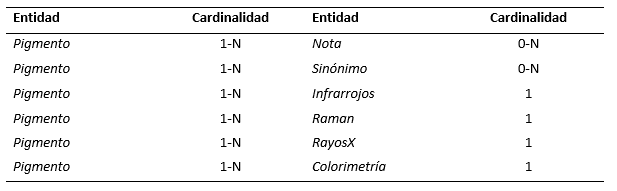
\includegraphics[scale=1]{imagenes/disenoBaseDatos/cardinalidades.png}
    \caption{Entidades y cardinalidades del modelo}
    \label{fig:cardinalidades}
\end{figure}

\subsubsection{Diagrama de Entidad Relación}

Una vez que hemos presentado tanto las entidades, como las cardinalidades y como están relacionadas las mismas, podemos mostrar como se relacionan las unas con las otras de una manera gráfica, que es presentado el diagrama de entidad relación de la base de datos. En este caso se ha decidido usar el formato de UML y no sigue las reglas estrictas del modelo de Entidad Relación, pero me parece que es más visual, la herramienta y el formato es más universal y entendible que el propio para expresar este tipo de contenidos. Podemos encontrar esto en la \textbf{Figura \ref{fig:diagramaER}}

\begin{figure}[H]
    \centering
    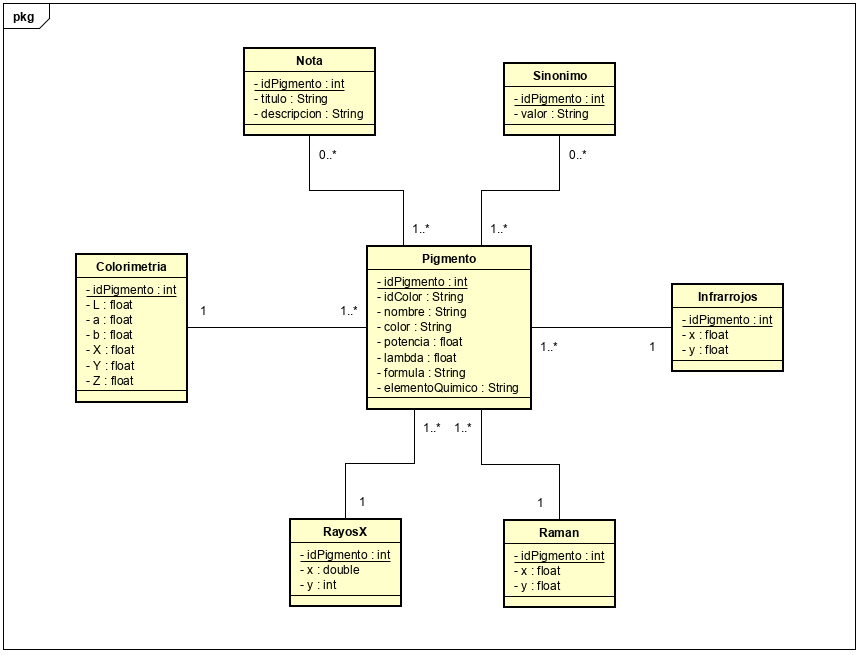
\includegraphics[scale=0.75]{imagenes/disenoBaseDatos/diagramaER.png}
    \caption{Diagrama de Entidad-Relación de la base de datos}
    \label{fig:diagramaER}
\end{figure}

En el diagrama podemos observar como la clave primaria de todas las relaciones es el id del pigmento en cuestión. Esto luego nos permitirá conectar unas relaciones con otras y buscar la información de una manera más adecuada. 

\textcolor{red}{mirar a ver las transformaciones y buscar un poco mas de teoría de diseño de la base de datos}

Una vez que tenemos el diseño de la base de datos podemos pasar a explicar la implementación de la misma, en lineas generales. 


\subsection{Implementación de la base de datos}
Una vez que tenemos la base de datos diseñada tenemos que implementarla dentro de nuestra aplicación. Para ello lo primero que tenemos que hacer es crear una clase auxiliar que nos permita la creación y en el futuro la conexión entre la propia aplicación y los datos almacenados en la base de datos. 

Para implementar la base de datos he optado por hacerlo de una manera más sencilla que la aprendida en la asignatura de SMOV. La base en realidad es la misma, pero la forma es la misma, bien es sabido que dentro de la informática podemos obtener los mismos resultados pero con algoritmos diferentes. En este caso vamos a realizar una mezcla entre uno de los patrones de acceso comentados al principio, DAO y los POJO.

Como hemos dicho en los capítulos anteriores, cada uno de los elementos de la base de datos, que en este caso son pigmentos, va a estar representado por un objeto típico de Java. Esta forma de representar los objetos para el almacenamiento de datos se denomina POJO (\textbf{P}lain \textbf{O}ld \textbf{J}ava \textbf{O}bjects).

Además cada vez que recuperemos los elementos de la base de datos lo hacemos devolviendo una lista de objetos del tipo adecuado. Por ejemplo para devolver todos y cada uno de los pigmentos que hay en la base de datos lo que hacemos es mandar la consulta al SGBD de SQLite y lo que nos devuelve es una lista de POJOs del tipo deseado. 

De esta manera podemos acceder de una manera sencilla a todos los atributos de los datos que acabamos de recuperar.

\subsubsection{¿Que son los POJO?} 

Dicho término \cite{pojo} fue acuñado por Martin Fowler, Rebecca Parsons y Josh MacKenzie en Septiembre del 2000. Se usa para referirse a un objeto Java que no tiene limitaciones de por requerir librerías ni clases externas. Son objetos simples y básicos de java, con atributos, funciones para recuperar los valores y para cambiarlos en caso necesario y nada más. Este tipo de objetos son muy utilizados cuando tenemos que convertir objetos entre diferentes lenguajes o cuando tenemos que serializarlos para enviarlos por la red. 

Idealmente y según dice la definición de los mismos, un objeto Java es POJO si cumple estos 3 requisitos:
\begin{itemize}
    \item No extiende de ninguna clase. 
        \begin{figure}[H]
        \lstinputlisting[style=customc]{capitulos/disenoBaseDatos/codigo/noExtiende.java}
        \label{fig:noExtiende}
        \end{figure}
    
    \item No implementa ninguna clase. 
        \begin{figure}[H]
        \lstinputlisting[style=customc]{capitulos/disenoBaseDatos/codigo/noImplementa.java}
        \label{fig:noImplementa}
        \end{figure}
        
    \item No contiene anotaciones. 
        \begin{figure}[H] 
        \lstinputlisting[style=customc]{capitulos/disenoBaseDatos/codigo/noAnotaciones.java}
        \label{fig:noAnotaciones}
        \end{figure}
\end{itemize}

Los POJO fueron inicialmente utilizados en J2EE para representar los JavaBeans, que son objetos java muy simples y que ofrecen servicios por la red. Se siguen utilizando aunque han cambiado un poco las formas de hacerlo. Ahora los POJO también son ampliamente utilizados para representar objetos JSON recibidos por parte de microservicios web y ser utilizados en un servidor. Este es uno de los muchos ejemplos de utilización real a día de hoy de los POJO. 

\subsubsection{Ejemplo}

Vamos a explicar con un sencillo ejemplo lo que son los POJO y como se hace la consulta de los mismos para luego mostrar la información dentro de la aplicación.

En este caso uno de los atributos que nos interesa son las diferentes notas que tiene cada uno de los pigmentos, para ello habrá una tabla con todas las notas de todos los pigmentos. Como hemos enseñado en el modelado conceptual, de cada una de las diferentes notas almacenamos y guardamos los siguientes datos: 
\begin{itemize}
    \item IdPigmento: para poder relacionar la nota con el pigmento, este dato es interno para la gestión de los datos. 
    \item Título: breve descripción.
    \item Descripción: contenido completo de la nota. 
    \item Fecha: fecha de creación de la misma. 
\end{itemize}

La descripción anterior la podemos encontrar representada por un POJO en el siguiente fragmento de cñodigo Java: 

\begin{figure}[H] 
\lstinputlisting[style=customc]{capitulos/disenoBaseDatos/codigo/notaPojo.java}
\label{fig:notaPojo}
\end{figure}





\subsection{Otras consideraciones}
Algunas otras decisiones de diseño que hemos tenido que tener en cuenta, y que afectan tanto al rendimiento de la aplicación como al diseño de la base de datos, son las siguientes:

\subsubsection{Diseño antiguo VS diseño actual}
En el diseño antiguo de la base de datos (\textbf{Figura \ref{fig:accessDesign}}), de manera resumida se tiene una tabla con una entrada para cada pigmento y esta entrada tiene un atributo que referencia a un fichero de datos. Por ejemplo si queremos obtener el difractograma de rayos X del pigmento número 3, nos va a referenciar a un fichero de texto que contiene aproximadamente unas 4000 líneas con 2 valores en cada línea. Es decir que en total vamos a tener unos 50 ficheros cada uno de 4000 líneas. Según el gestor de almacenamiento de Windows estos ficheros tienen un tamaño medio de unos 30 Kb. En total tenemos unos 150 ficheros lo que hace que el total de los ficheros si los tuviéramos que almacenar dentro de la base de datos para su posterior procesado, además de tener aparte la instancia de la base de datos creada supondría un aumento de unos 5Mb en la aplicación.

\begin{figure}[H]
    \centering
    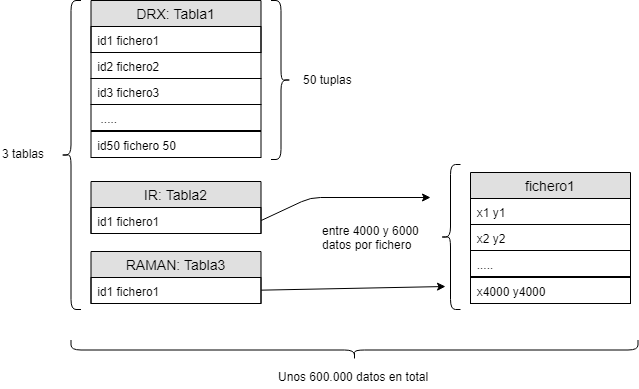
\includegraphics[scale=0.75]{imagenes/disenoBaseDatos/accessDesign.png}
    \caption{Diseño propuesto en Access de la Base de Datos}
    \label{fig:accessDesign}
\end{figure}

En el diseño que yo he propuesto (\textbf{Figura \ref{fig:sqliteDesign}}) lo que tenemos son 3 tablas, cada una de 200.000 entradas (50 x 4000 en el peor de los casos) donde tenemos disponibles todos y cada uno de los datos. Además una de las ventajas de esta forma es que la aplicación no tiene que hacer tantas operaciones de entrada salida para procesar todos los datos al realizar las consultas. Con el diseño propuesto solo se procesan una única vez para poder cargar y generar la base de datos. 

\begin{figure}[H]
    \centering
    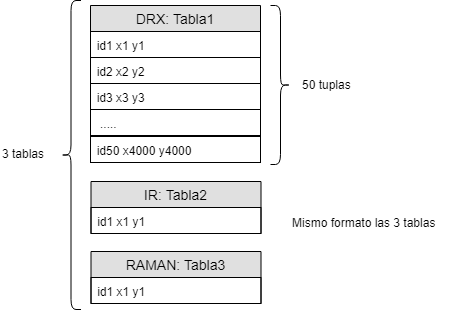
\includegraphics[scale=0.75]{imagenes/disenoBaseDatos/sqliteDesign.png}
    \caption{Diseño propio de la base de datos}
    \label{fig:sqliteDesign}
\end{figure}


\subsubsection{Código frente a eficacia}

Otro de los problemas es la eficacia y el diseño frente a la limpieza y entendibilidad del código. Podemos implementar la solución de dos maneras diferentes. 

La primera es creando una única base de datos con todas las tablas y todas las operaciones necesarias. El problema es que esa base de datos y las operaciones se tienen que crear en una única clase que se encarga de ello, esta clase va a ser relativamente grande y uno de los principios de diseño que por ejemplo podemos encontrar en el Libro Clean Code \cite{cleanCode} es que las clases tienen que ser pequeñas, autocontenidas y hacer una única cosa. Sin embargo nuestra clase va a crear una base de datos, inicializar 4 tablas y ofrecer todos los métodos de acceso y modificación de todas las tablas.

De esta forma el código se ve afectado pero sin embargo el diseño de la base de datos y la eficacia de las consultas no se ve afectada.

La otra manera es crear una clase para cada una de las tablas, pero de esta manera tendríamos una base de datos por tabla, lo que no concuerda con el diseño propuesto de la base de datos y además tendríamos que procesar las consultas via software usando la JVM lo cual puede traducirse en un decremento de la eficiencia de la aplicación. 

La solución por la que se ha optado es la primera. 
 \newpage
\newpage


% empezamos la bibliografía
\begin{thebibliography}{X}

\bibitem{manifiestoAgil}
\textbf{Manifiesto Ágil}. \textit{Manifiesto ágil con los principios de agilidad software}. \\
\small{\url{https://agilemanifesto.org/iso/es/manifesto.html}}

\bibitem{atlassian}
\textbf{Attlasian Company}. \textit{Información de la empresa líder en herramientas de PM}. \\
\small{\url{https://es.atlassian.com/}}

\bibitem{kanbanAtlassian}
\textbf{Kanban - Atlassian}. \textit{Información de Kanban de Atlassian}. \\
\small{\url{https://es.atlassian.com/agile/kanban}}

\bibitem{scrumAtlassian}
\textbf{Scrum - Atlassian}. \textit{Información de Scrum de Atlassian}. \\
\small{\url{https://es.atlassian.com/agile/scrum}}

\bibitem{jiraAtlassian}
\textbf{Jira}. \textit{Información de Jira de Atlassian}. \\
\small{\url{https://es.atlassian.com/software/jira}}

\bibitem{taiga}
\textbf{Taiga Software}. \textit{Software para control de proyectos ágiles}. \\
\small{\url{https://tree.taiga.io/discover}}

\bibitem{sonarqube}
\textbf{SonarQube}. \textit{Software para el control de la calidad del software}. \\
\small{\url{https://www.sonarqube.org/features/clean-code/}}

\bibitem{sonarlint}
\textbf{SonarLint}. \textit{Plugin agregado de SonarQube para el control de la calidad en el IDE}. \\
\small{\url{https://www.sonarlint.org/}}

\bibitem{jenkins}
\textbf{Jenkins}. \textit{Softwre para la integración continua y la entrega continua de software}. \\
\small{\url{https://jenkins.io/}}

\bibitem{androidstudio}
\textbf{Android Studio}. \textit{Entorno de desarrollo integrado para programación de aplicaciones multiplataforma}. \\
\small{\url{https://developer.android.com/studio}}

\bibitem{github}
\textbf{Github}. \textit{Software de control de versiones en la nube}. \\
\small{\url{https://github.com/}}

\bibitem{sqlite}
\textbf{SQLite}. \textit{SGBD ligero integrado en Android}. \\
\small{\url{https://www.sqlite.org/index.html}}

\bibitem{overleaf}
\textbf{Overleaf}. \textit{Sistema de composición de textos basado en \LaTeX}. \\
\small{\url{https://es.overleaf.com/}}

\bibitem{confluence}
\textbf{Confluence}. \textit{Sistema de documentación en la nube propietario de Atlassian}. \\
\small{\url{https://es.atlassian.com/software/confluence}}

\bibitem{docker}
\textbf{Docker}. \textit{Sistema de contenedores open source}. \\
\small{\url{https://www.docker.com/why-docker}}

\bibitem{gradle}
\textbf{Gradle}. \textit{Sistema de construcción de proyectos y gestor de dependencias}. \\
\small{\url{https://gradle.org/}}

\bibitem{gitflow}
\textbf{Gitflow - Atlassian}. \textit{Gitflow worflow de la empresa líder en Agilidad}. \\
\small{\url{https://es.atlassian.com/git/tutorials/comparing-workflows/gitflow-workflow}}

\bibitem{balsamiq}
\textbf{Balsamiq Mocuk Up}. \textit{Página principal de Balsamiq}. \\
\small{\url{https://balsamiq.com/wireframes/}}



\end{thebibliography}
\end{document}